\chapter{LoRa}

\section{Description}

LoRa (Long Range) is a wireless communication technology that allows for long-distance data transmission with low power consumption, making it ideal for Internet of Things (IoT) applications such as remote monitoring, smart agriculture, and industrial automation. The Portenta H7 Vision Shield includes a LoRa module to facilitate these long-range communication capabilities. \cite{connecting_to_ttn_portenta_vision_shield:2024}

\textbf{Key Features:}
\begin{itemize}
	
	\item \textbf{Integrated LoRa Module:} The Portenta H7 Vision Shield comes with an integrated LoRa module, enabling long-distance communication over several kilometers while using minimal power. This makes it suitable for IoT applications that require reliable, wide-area communication. 
	
	\item \textbf{Low Power Consumption:} The LoRa module is optimized for low power usage, ensuring that devices can operate for extended periods without needing frequent recharges, making it ideal for battery-powered applications. 
	
	\item \textbf{Wide Range:} The Portenta H7 Vision Shield’s LoRa module provides communication capabilities over long distances, typically up to 10 km in rural areas or 1-3 km in urban environments, depending on obstacles and interference.  \cite{connecting_to_ttn_portenta_vision_shield:2024}
	
\end{itemize}

\section{Specific Module}
The LoRa functionality in the Portenta H7 Vision Shield is powered by an integrated Semtech SX1276 transceiver, which is capable of both long-range communication and low-power operations. The module operates on the ISM band and is compatible with the LoRaWAN protocol, allowing seamless integration into LoRa networks such as The Things Network (TTN). \cite{connecting_to_ttn_portenta_vision_shield:2024}

\section{Specification}
\textbf{LoRa Module} = \SHELL{LoRa\_MOD} 

\begin{itemize}
	
	\item The LoRa module on the Portenta H7 operates in the sub-GHz frequency range, typically 868 MHz (Europe) or 915 MHz (North America).
	\item It is fully integrated into the Vision Shield, eliminating the need for additional hardware to enable LoRa communication.
	\item The LoRa module supports the LoRaWAN protocol, allowing devices to communicate with LoRa gateways for IoT network integration.
	\item It provides a communication range of up to 10 km in open space and up to 3 km in urban environments.
	\item The module is programmable via the Arduino IDE, allowing for easy setup and configuration for LoRa communication. \cite{connecting_to_ttn_portenta_vision_shield:2024}
	
\end{itemize}


\section{Simple Code}
In the listing  ~\ref{Simplewebserver}, the wifi module is initialized and created a server.

{
	\captionof{code}{Simplewebserver}\label{Simplewebserver}
	\ArduinoExternal{}{../Code/LORA/Simplewebserver.ino}
}



\section{EXAMPLES}

\subsection{Connecting the Portenta Vision Shield to TTN Using LoRa}
This tutorial explains how to connect your Portenta H7 to The Things Network (TTN) using the the Portenta Vision Shield's LoRa® Connectivity feature. \cite{connecting_to_ttn_portenta_vision_shield:2024}

\subsubsection{Overview}
This tutorial explains how to connect your Portenta H7 to The Things Network (TTN) using the the Portenta Vision Shield's LoRa Connectivity feature. A data communication channel will be enabled between the H7 and a TTN application that will be configured on your TTN console. \cite{connecting_to_ttn_portenta_vision_shield:2024}

\subsubsection{Goals}
\begin{itemize}
	\item About LoRaWAN and The Things Network,
	\item About creating a TTN application, 
	\item How to establish a connection between the Portenta H7 and the TTN. \cite{connecting_to_ttn_portenta_vision_shield:2024}
\end{itemize}

\subsubsection {Required Hardware and Software}
\begin{enumerate}
	\item Portenta H7
	\item USB-C cable (either USB-A to USB-C or USB-C to USB-C)
	\item Arduino IDE 1.8.13+ or Arduino Pro IDE 0.0.4+
	\item Portenta Vision Shield - LoRa
	\item 1x Dipole Pentaband antenna or a UFL Antenna of the H7 
	\item An account with The Things Network \cite{connecting_to_ttn_portenta_vision_shield:2024}
\end{enumerate}

\subsubsection {Updating the LoRa Module Firmware}
To be able to use the LoRa functionality, we need to first update the firmware on the LoRa modem. This can be done through Arduino IDE by running a sketch included in the examples from the MKRWAN library.

\begin{enumerate}
	\item Connect the Portenta H7 and the Portenta Vision Shield - LoRa to your computer and open the Arduino IDE.
	\item Install/update the \SHELL{MKRWAN} library from Arduino IDE menu \SHELL{Tools > Manage Libraries}. Type "MKRWAN" to find the library and click 'Install' or 'Update' if necessary. This library provides all the APIs to communicate with LoRa® and LoRaWAN networks.
	\item Open the \SHELL{MKRWANFWUpdate standalone} sketch from the Arduino IDE menu: \SHELL{File > Examples > MKRWAN}.
	\item Upload the sketch. \cite{connecting_to_ttn_portenta_vision_shield:2024}
\end{enumerate}

	\begin{figure}
		\begin{center}
			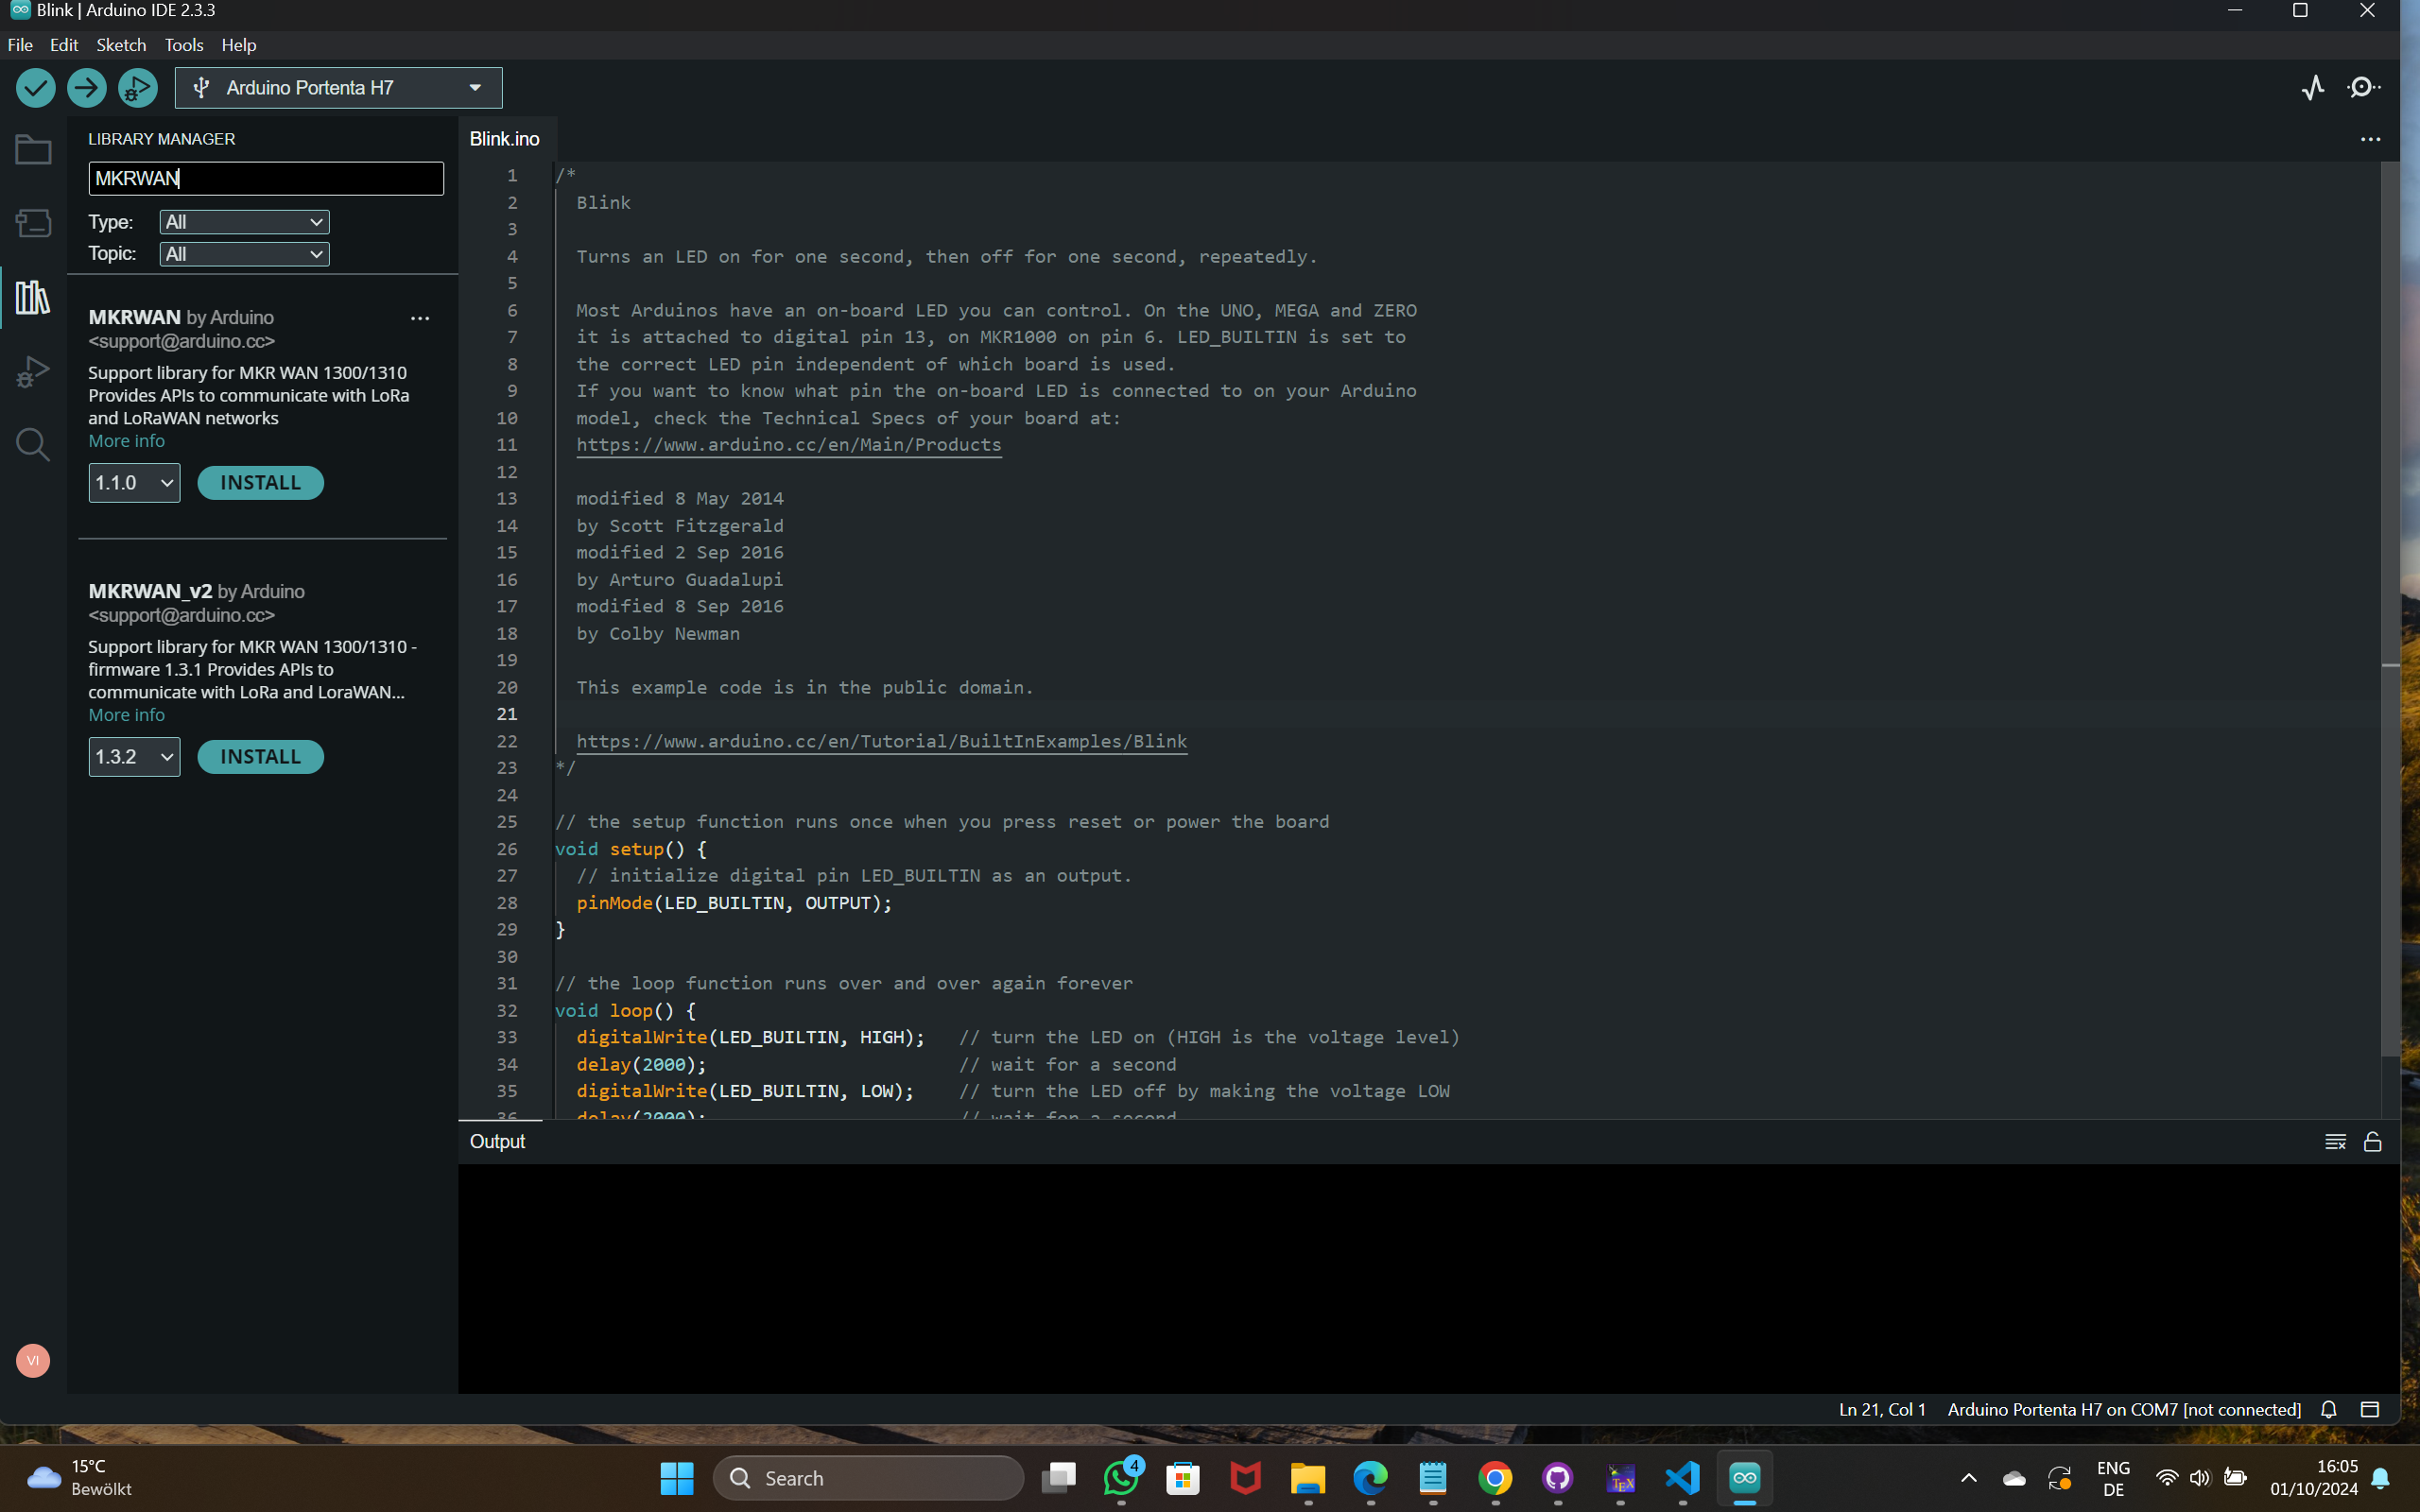
\includegraphics[width=0.7\linewidth]{Images/LORA/InstallMKRWAN.png}
			\caption{Install MKRWAN}
			\label{Install MKRWAN}\cite{connecting_to_ttn_portenta_vision_shield:2024}
		\end{center}
	\end{figure}
	
	\begin{figure}
		\begin{center}
			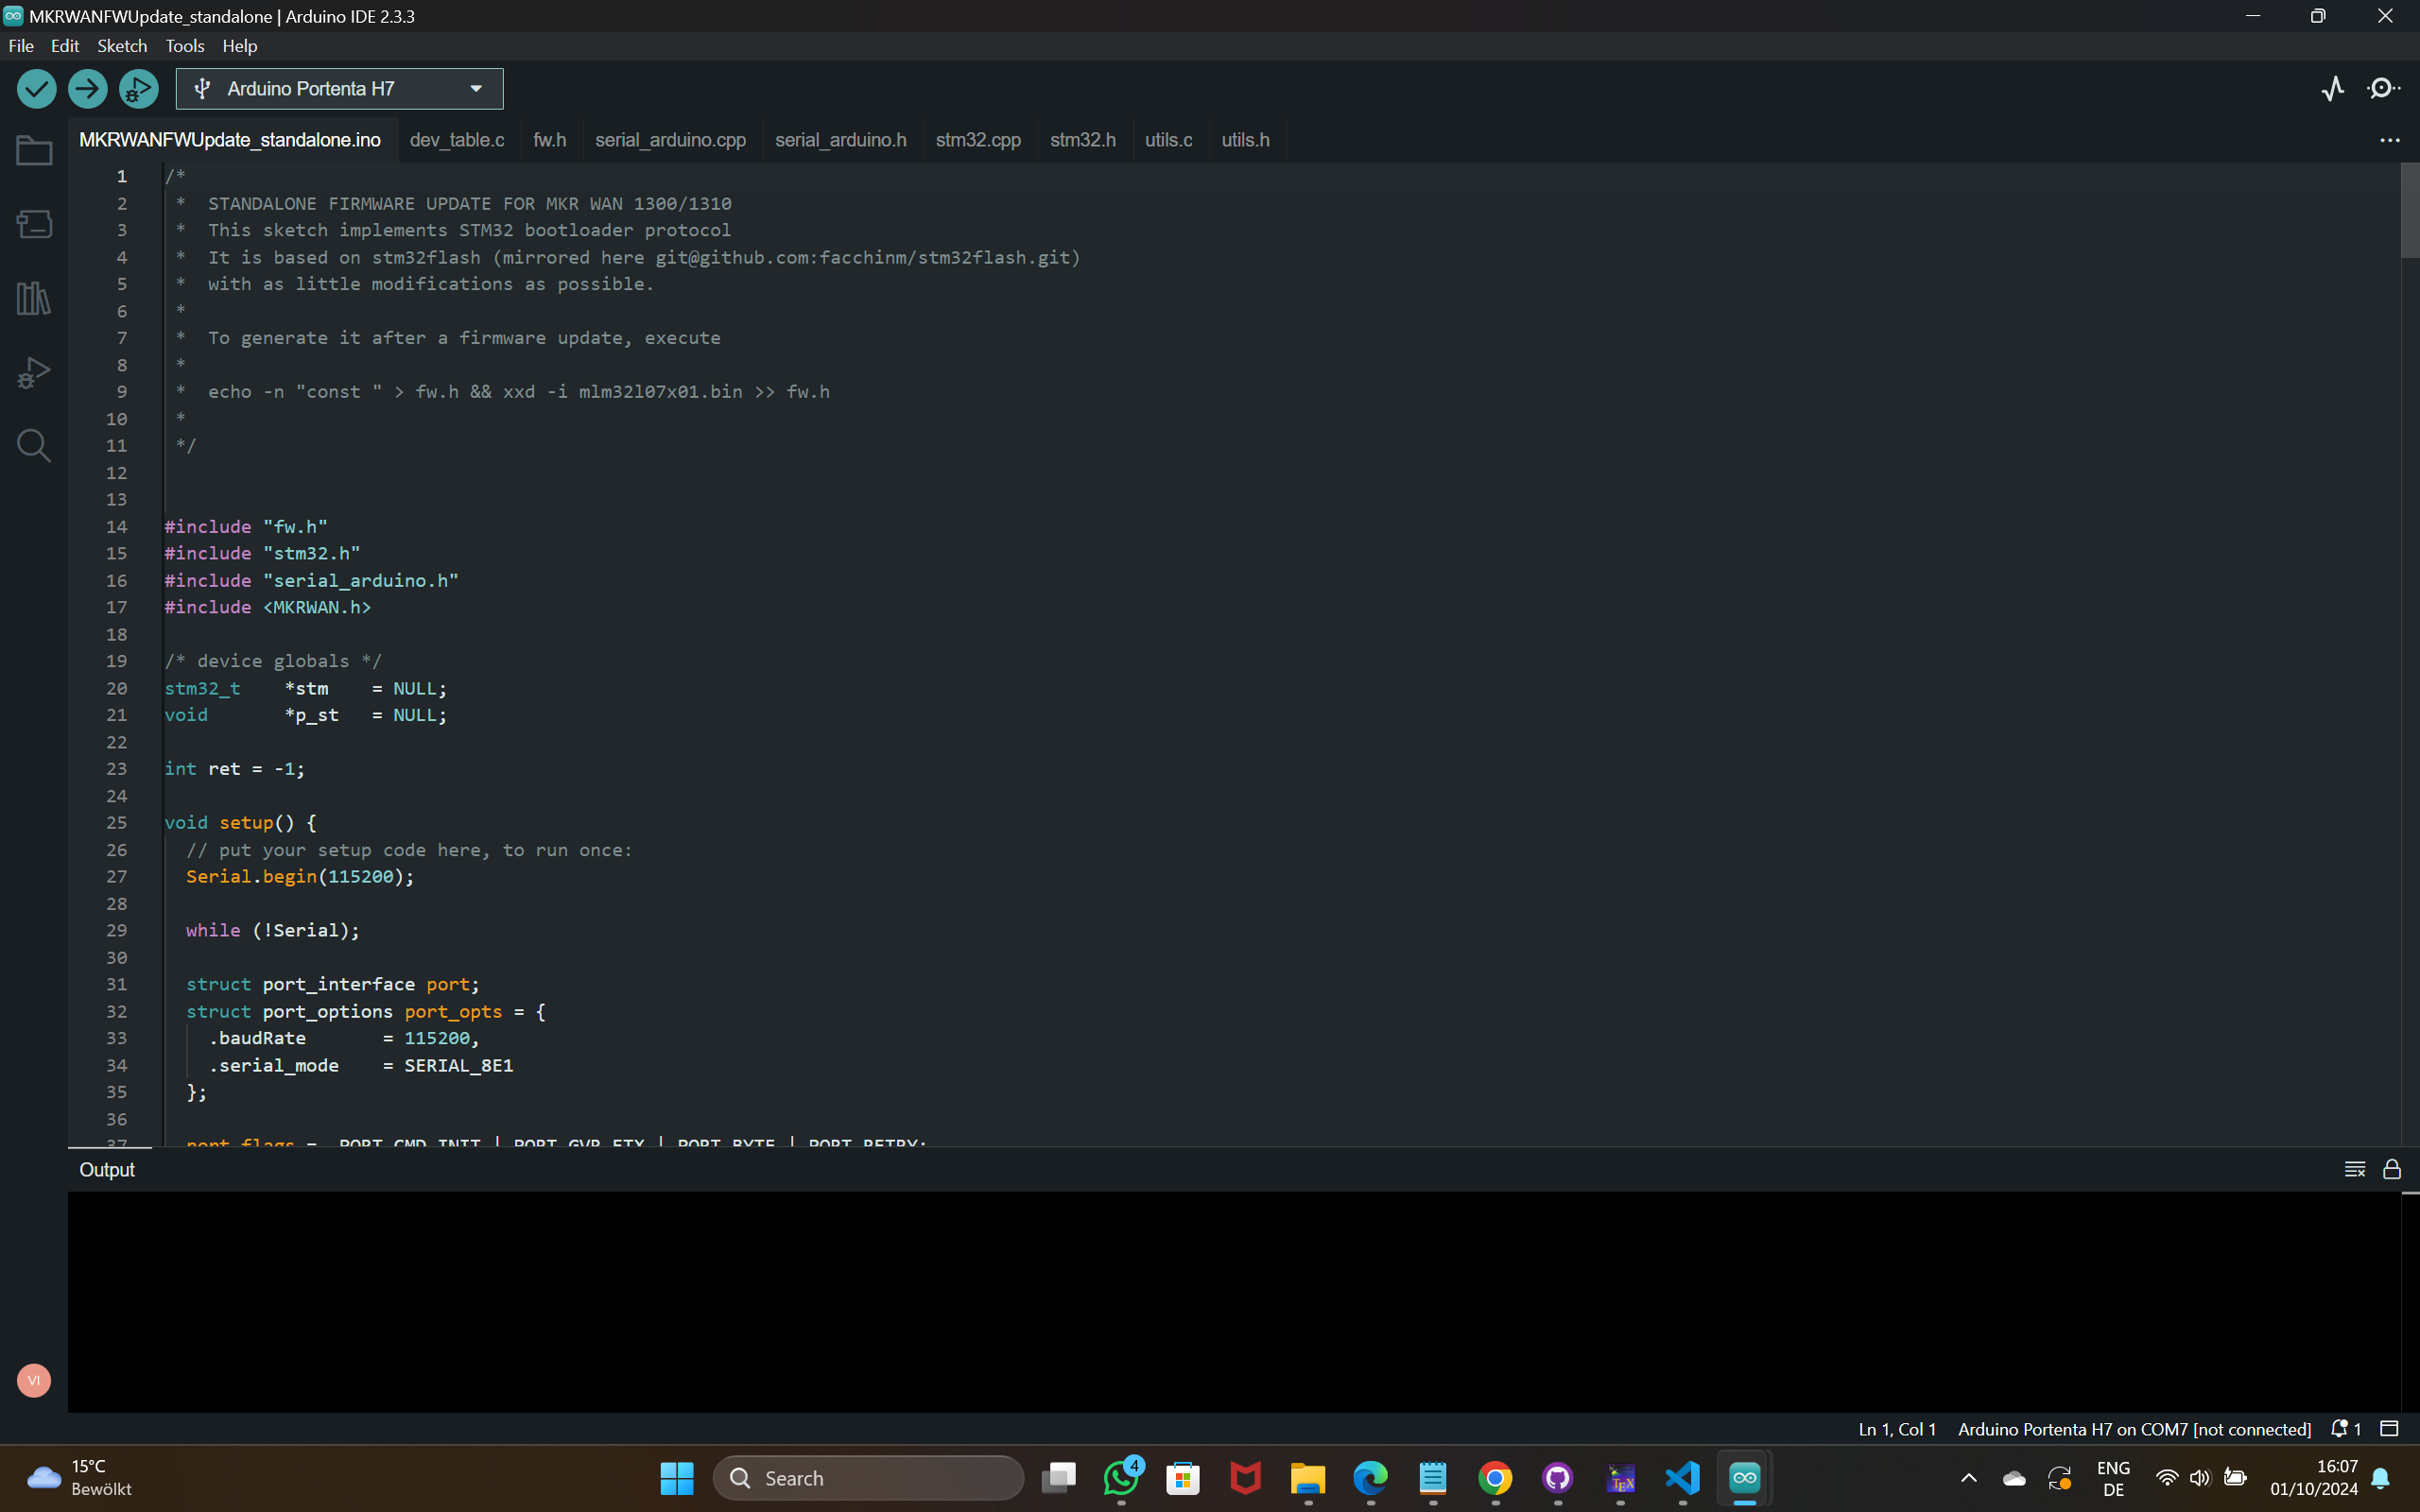
\includegraphics[width=0.7\linewidth]{Images/LORA/MKRWANStandalone.png}
			\caption{MKRWAN Standalone}
			\label{MKRWAN Standalone}\cite{connecting_to_ttn_portenta_vision_shield:2024}
		\end{center}
	\end{figure}

	\textbf{Open the Serial Monitor and wait for the update to be confirmed.}
	
	\begin{figure}
		\begin{center}
			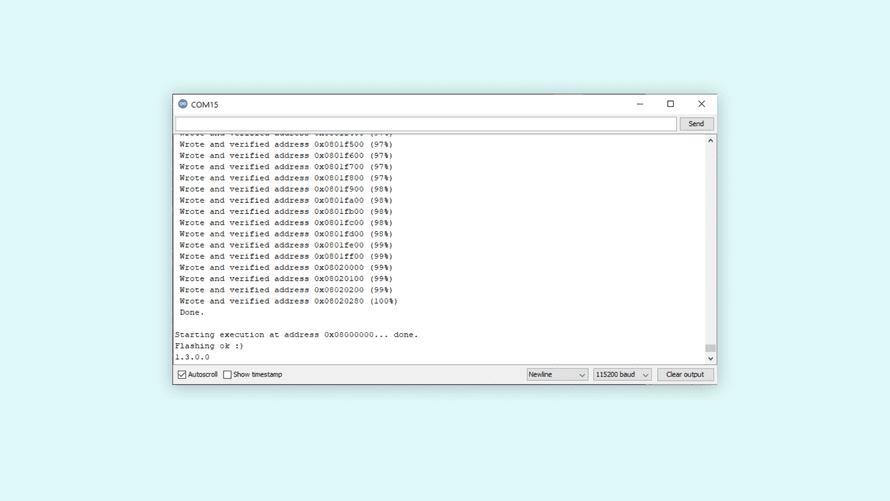
\includegraphics[width=0.7\linewidth]{Images/LORA/SerialMonitor.png}
			\caption{SerialMonitor}
			\label{SerialMonitor}\cite{connecting_to_ttn_portenta_vision_shield:2024}
		\end{center}
	\end{figure}
	
	
\subsubsection{Connecting to the TTN}
The Portenta Vision Shield - LoRa can be connected to the TTN and can transmit data to other devices connected to this network through a secure channel. This channel is nothing but an application on the TTN network dedicated for your board. In this tutorial, you will be guided through a step-by-step process of setting up your Portenta board and the Vision Shield - LoRa to communicate with a TTN application. As stated before, to be able to follow this guide, you need to be under coverage of one of the TTN gateways. You can check for the coverage now if you have not done so yet.
\begin{itemize}
	
	\item \textbf{1. Setting up the Environment} First choose your region. Next, sign in with your The Things Network account. If you do not have an account, create a new one on the login page. Then fill all the required fields to complete a new registration. ~\ref{Things Network} \cite{connecting_to_ttn_portenta_vision_shield:2024}
	
	\begin{figure}
		\begin{center}
			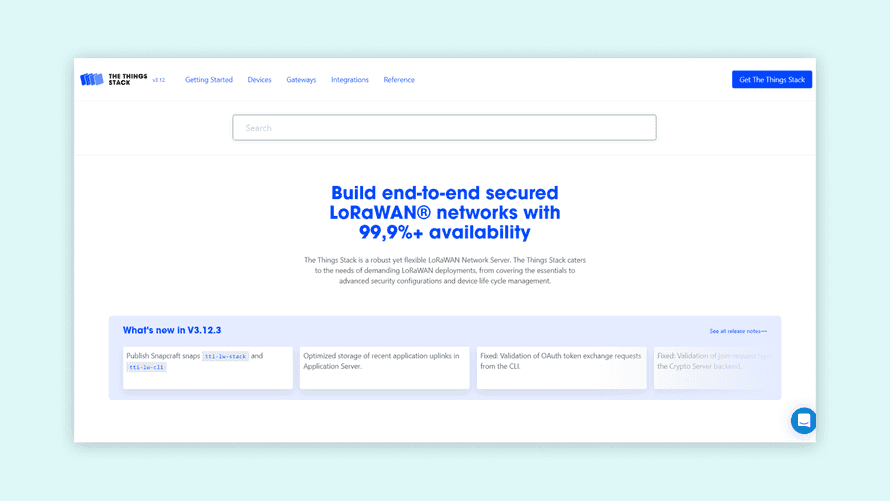
\includegraphics[width=0.7\linewidth]{Images/LORA/ThingsNetwork.png}
			\caption{Things Network}
			\label{Things Network}\cite{connecting_to_ttn_portenta_vision_shield:2024}
		\end{center}
	\end{figure}
	
	\item \textbf{2. Creating an App on TTN} Once you have created an account with TTN, you need to create a \SHELL{TTN application}. An application provides a way to aggregate data from different devices, and then use these data with other 3rd party integrations. After signing in, click on \SHELL{Create an application, or Go to applications} if you already have created one. ~\ref{SelectApplication} \cite{connecting_to_ttn_portenta_vision_shield:2024}
	
	\begin{figure}
		\begin{center}
			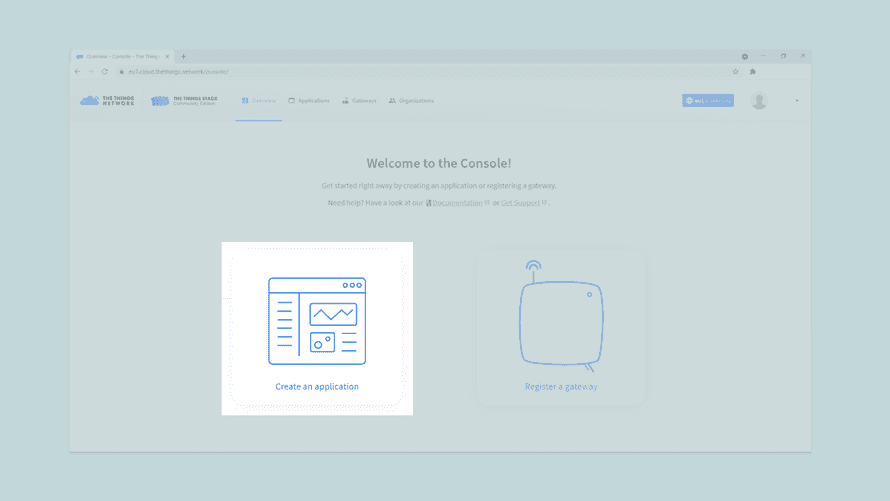
\includegraphics[width=0.7\linewidth]{Images/LORA/SelectApplication.png}
			\caption{Select Application}
			\label{Select Application} \cite{connecting_to_ttn_portenta_vision_shield:2024}
		\end{center}
	\end{figure}
	
	Here you will have a list of all your applications. Now create your first app by pressing the Create an application button.
	
	You have now to fill only the first two fields:
	
	\begin{enumerate}
		\item The first one is the Owner of your app, it will automatically have you as the owner.
		\item The second one is the ID of your app: this must be lowercase and without spaces.
	\end{enumerate}
	
	\begin{figure}
		\begin{center}
			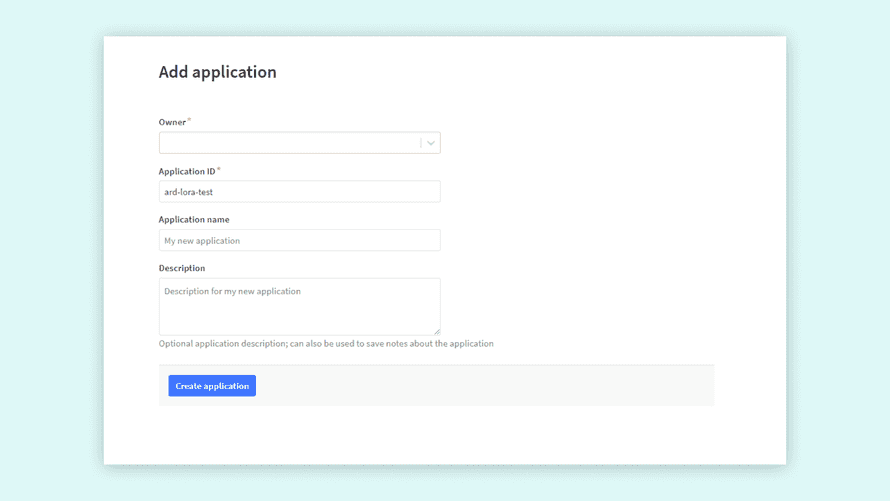
\includegraphics[width=0.7\linewidth]{Images/LORA/AddingApplication.png}
			\caption{AddingApplication}
			\label{AddingApplication} \cite{connecting_to_ttn_portenta_vision_shield:2024}
		\end{center}
	\end{figure}
	
	After completing these two fields, press the "Create application" button located at the bottom left corner of the page. The dashboard will then show you an overview of the newly created app. 
	
	\begin{figure}
		\begin{center}
			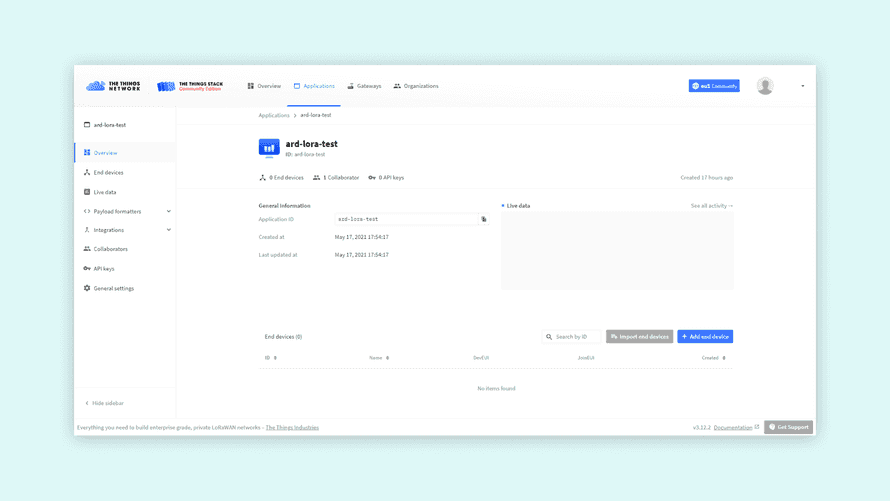
\includegraphics[width=0.7\linewidth]{Images/LORA/AppParameter.png}
			\caption{AppParameter}
			\label{AppParameter} \cite{connecting_to_ttn_portenta_vision_shield:2024}
		\end{center}
	\end{figure}
	
	Let's take a closer look at these sections:
	\begin{enumerate}
		\item \textbf{Application Overview:} in order to use this app, you will need the Application ID and a device specific AppKey. An EUI is a globally unique identifier for networks, gateways applications and devices. The EUIs are used to identify all parts of the LoRaWAN® inside the backend server.
		\item \textbf{End devices:}here you can see and manage all the associated devices (e.g. your Portenta H7 with Portenta Vision Shield - LoRa, Arduino MKR WAN 1300 or MKR WAN 1310), or proceed with the registration of a new one. Registering a new device lets you generate an AppEUI and an AppKey.
		\item \textbf{Collaborators:} here you can see and manage all the app collaborators, to integrate with other collaborative platforms or to manage access rights to the app with other TTN registered profiles.
		\item \textbf{API keys:} here you can create an API key, it is the most sensible information. It is basically the key to gain access to your app, so keep it safe.
	\end{enumerate}
	
	\item \textbf{3. Configuring the Portenta Vision Shield} It iss now time to connect your Portenta H7 and Portenta Vision Shield - LoRa to TTN. You will need to upload code to the board, so, as you probably already know, there are two options:
	
	Use the Arduino Cloud Editor
	
	Use the Arduino IDE, (this is the option this guide will follow)
	
	Plug the Portenta Vision Shield - LoRa to the Portenta H7 and them to your PC through the USB port. Be sure to have selected the right board "Arduino Portenta H7 (M7 core)" and the right port. ~\ref{MCore} \cite{connecting_to_ttn_portenta_vision_shield:2024}
	
	\begin{figure}
		\begin{center}
			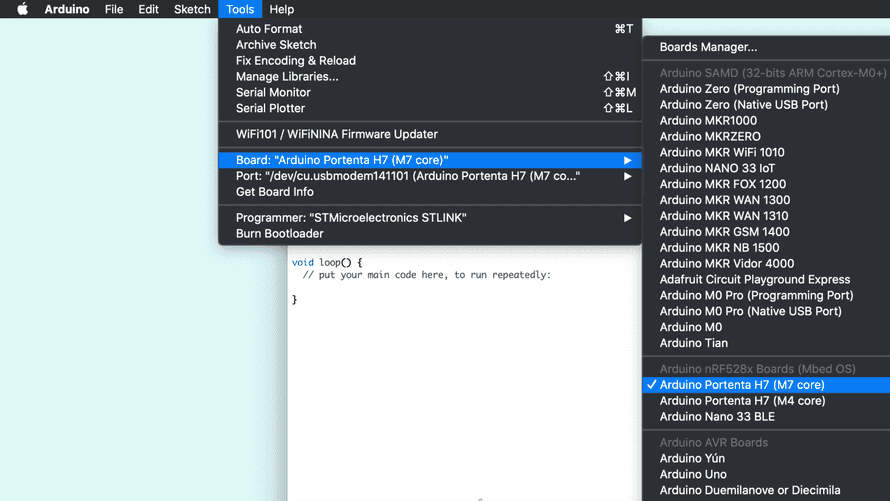
\includegraphics[width=0.7\linewidth]{Images/LORA/MCore.png}
			\caption{MCore}
			\label{MCore}
		\end{center}
	\end{figure}
	
	The LoRa module on the Portenta Vision Shield - LoRa can be accessed by using the \SHELL{MKRWAN library}(if you cannot find it in your examples list, you can go to \SHELL{Tools > Library Manager} and type "MKRWAN library" to install it). This library provides all the APIS to communicate with LoRa and LoRaWAN networks and can be installed from the library Manager. The first code you need to upload and run is from the \SHELL{MKRWAN} library, and its name is \SHELL{FirstConfiguration}. 
	
	\begin{figure}
		\begin{center}
			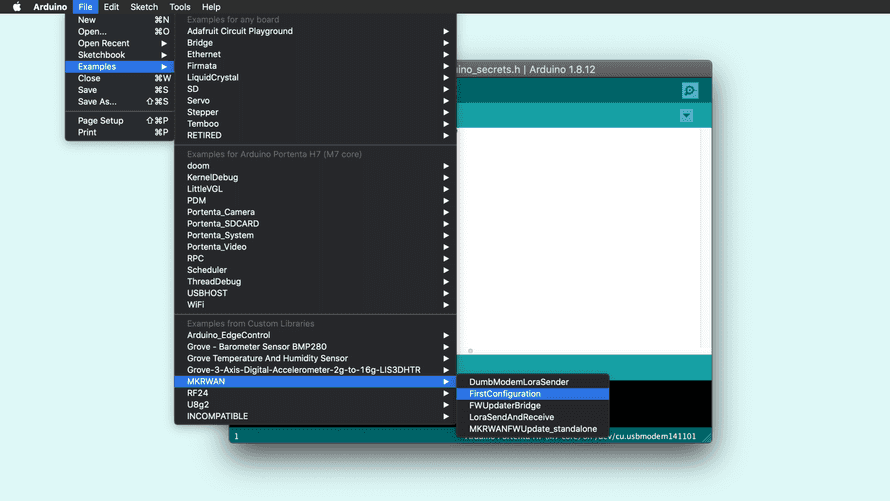
\includegraphics[width=0.7\linewidth]{Images/LORA/UploadCode.png}
			\caption{UploadCode}
			\label{UploadCode} \cite{connecting_to_ttn_portenta_vision_shield:2024}
		\end{center}
	\end{figure}
	
	The only line you may need to change before uploading the code is the one that sets the frequency. Set the frequency code according to your country if needed. You can find more information about frequency by country at this TTN link.
	
	\begin{lstlisting}[language=C++, frame=single, numbers=left, basicstyle=\ttfamily\small]
		// change this to your regional band (eg. US915, AS923, ...)
		if (!modem.begin(EU868)) {    ...
	\end{lstlisting}
	
	Once you have added to the sketch the frequency according to your country, you can upload it to the board. Then, when the upload is completed, open the Serial Monitor. The following details will show up:
	
	\begin{lstlisting}[language=C++, frame=single, numbers=left, basicstyle=\ttfamily\small]
		Your module version is: ARD-078 1.2.1
		Your device EUI is: a8xxxxxxxxxxxxxx
		Are you connecting via OTAA (1) or ABP (2)?
	\end{lstlisting}
	
	In order to select the way in which the board is going to connect with TTN (OTAA or ABP), you need to configure it on the TTN portal. You will see which option you should select in the following steps.
	
	\item \textbf{4. Registering the Portenta on TTN} Before your Portenta H7 can start communicating with the TTN, you need to register the board with an application. Go back to the TTN portal and scroll to \SHELL{End devices} section on your Application dashboard, then click \SHELL{Add end device.} ~\ref{RegisteringDevice} \cite{connecting_to_ttn_portenta_vision_shield:2024} 
	
	\begin{figure}
		\begin{center}
			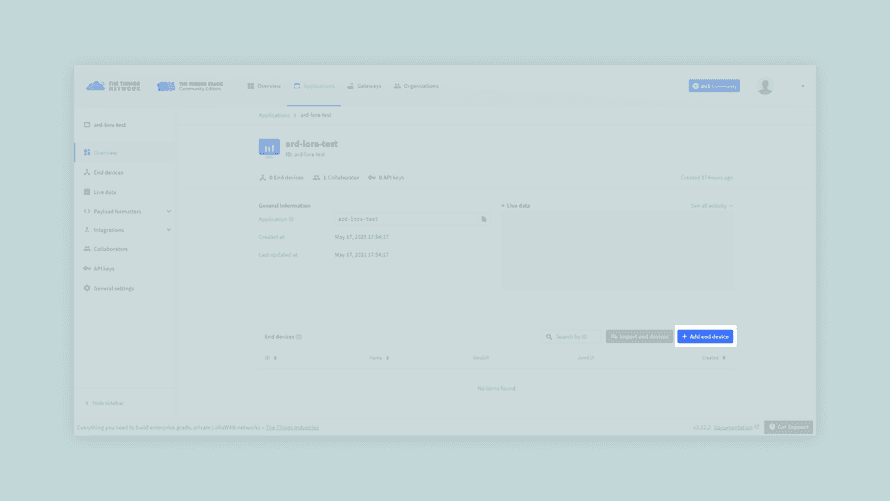
\includegraphics[width=0.7\linewidth]{Images/LORA/RegisteringDevice.png}
			\caption{RegisteringDevice}
			\label{RegisteringDevice} \cite{connecting_to_ttn_portenta_vision_shield:2024}
		\end{center}
	\end{figure}
	
	On the registration page, first you have to fill in information about your board. Select brand Arduino SA, and Portenta Vision Shield - LoRa as the model. Hardware and firmware versions will automatically be set to the newest ones. Then set your preferred region.
	
	\begin{figure}
		\begin{center}
			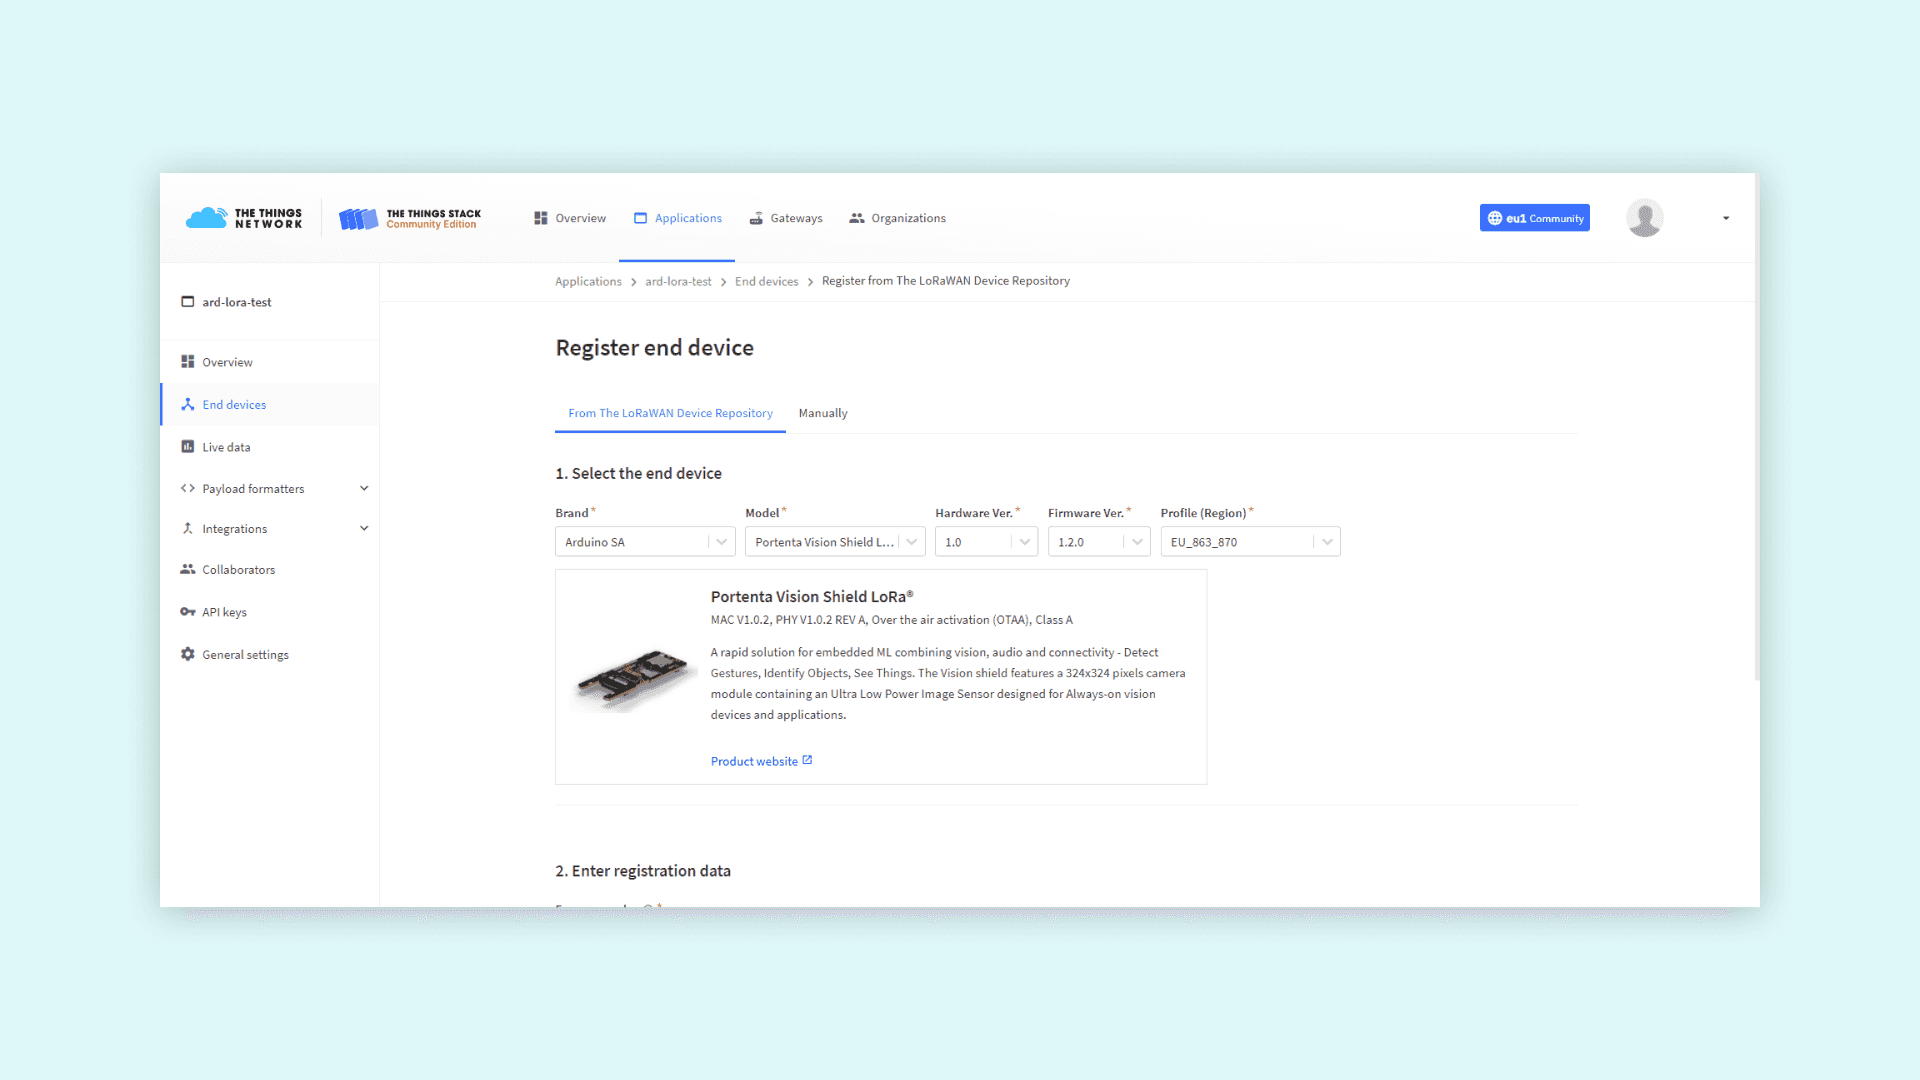
\includegraphics[width=0.7\linewidth]{Images/LORA/DeviceEUI.png}
			\caption{RegisteringDevice}
			\label{RegisteringDevice} \cite{connecting_to_ttn_portenta_vision_shield:2024}
		\end{center}
	\end{figure}
	
	In the second step of registering the device, fill in \SHELL{End device ID} and \SHELL{End device ID}. You can click the generate button next to the AppKey field to generate an app key for this device. Similarly, you can press the button next to the AppEUI field to make it all zeros, or enter your own AppEUI.
	
	\SHELL{Note:} The Device ID must be lowercase and without spaces. The \SHELL{DevEUI} should be copied from the Serial Monitor. 
	
	\begin{figure}
		\begin{center}
			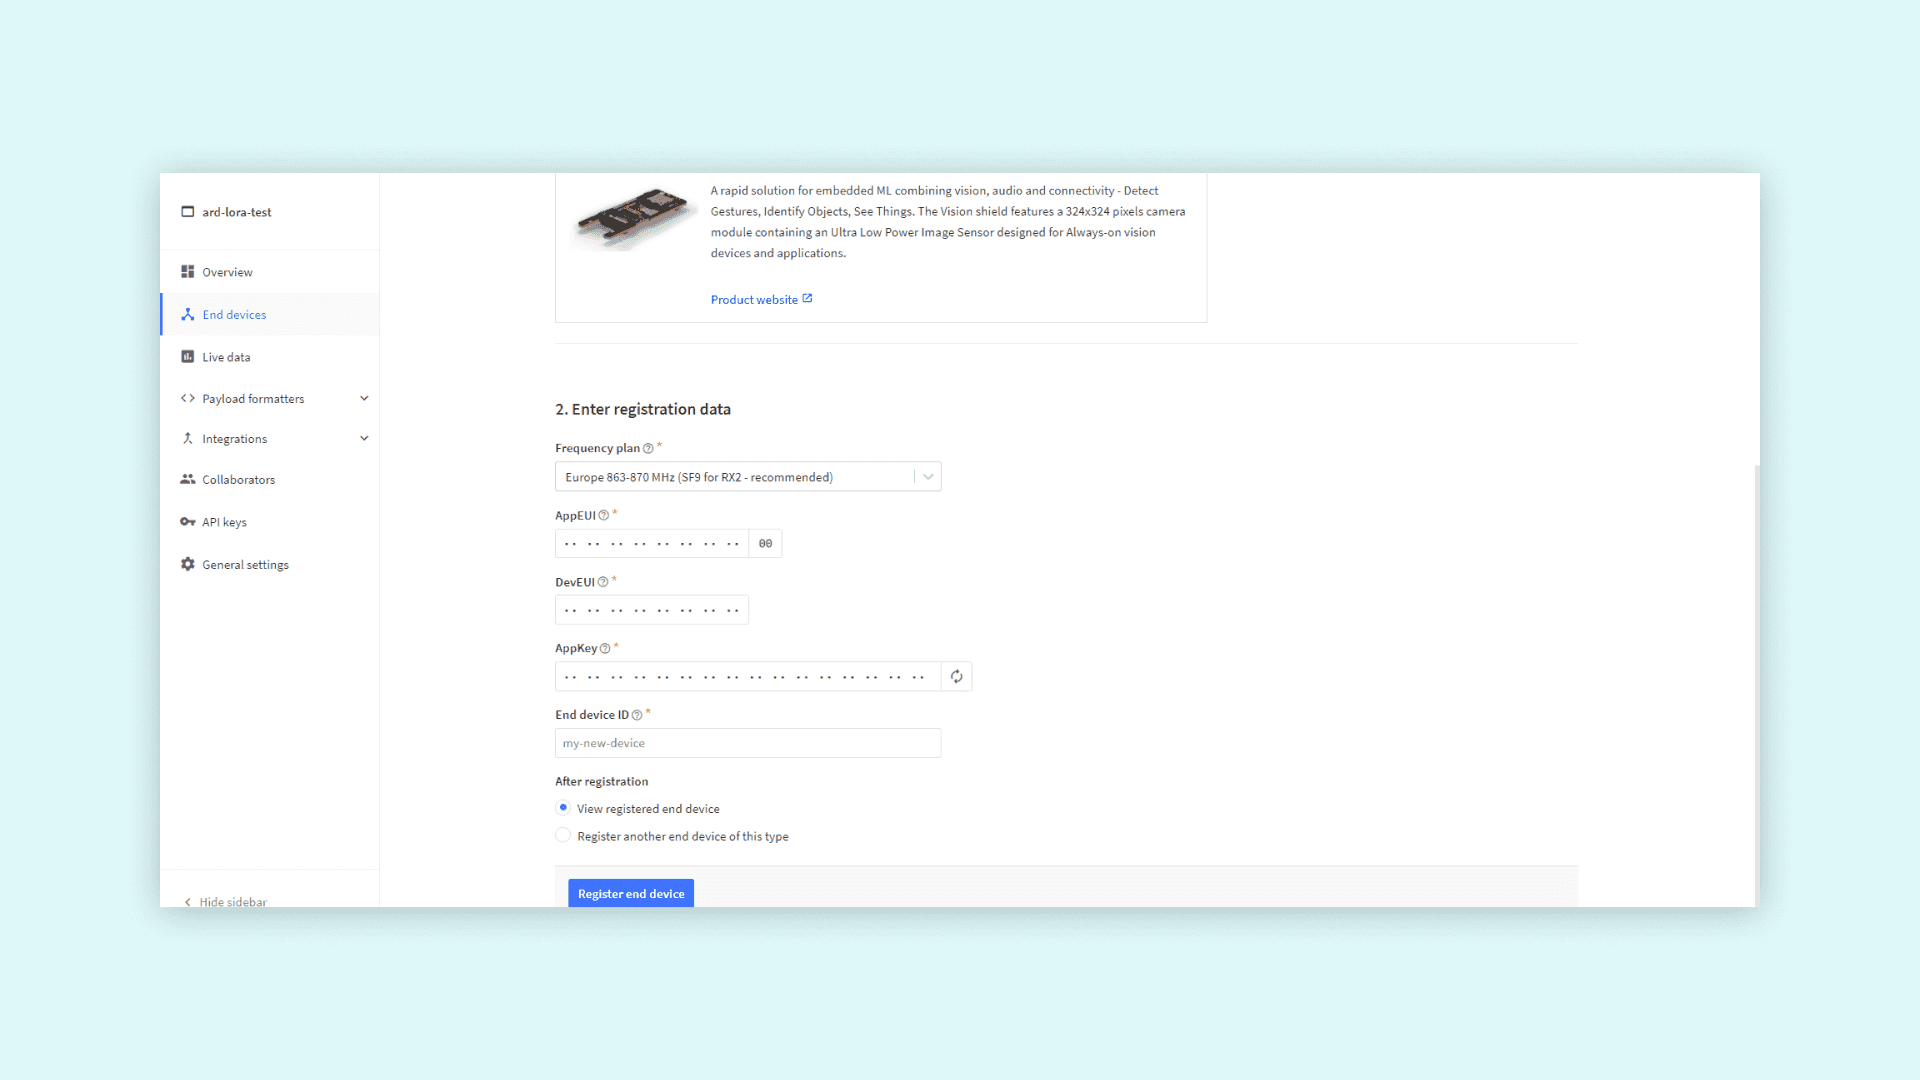
\includegraphics[width=0.7\linewidth]{Images/LORA/Secondstep.png}
			\caption{Secondstep}
			\label{Secondstep} \cite{connecting_to_ttn_portenta_vision_shield:2024}
		\end{center}
	\end{figure}
	
	After pressing the Register button, your board will show up on the \SHELL{Device Overview} page. You can now see all the information needed to complete the Arduino setup. 
	
	\begin{figure}
		\begin{center}
			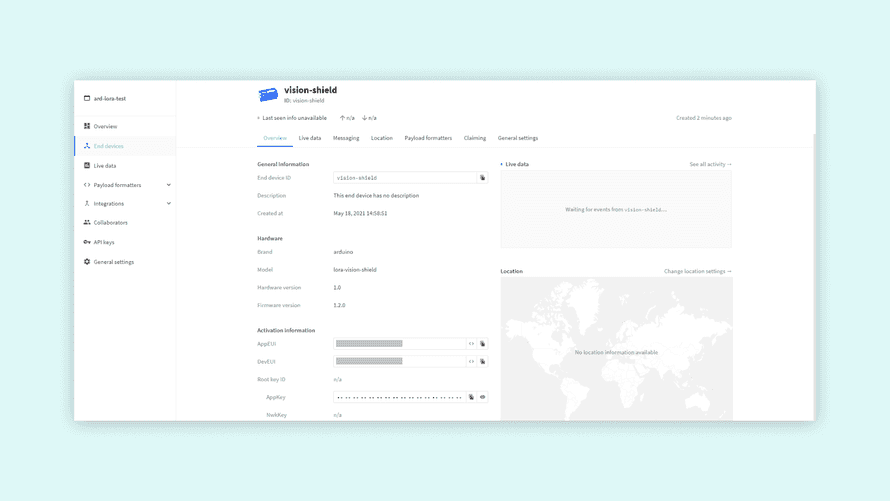
\includegraphics[width=0.7\linewidth]{Images/LORA/Overview.png}
			\caption{Secondstep}
			\label{Secondstep} \cite{connecting_to_ttn_portenta_vision_shield:2024}
		\end{center}
	\end{figure}
	
	\item \textbf{5. Connecting to TTN} Once your board has been registered you can send information to TTN. Let's come back to the Serial Monitor and proceed. It will ask for: ~\ref{Select-board-h7}
	
	\begin{enumerate}
		\item Activation mode (that, in this case, is OTAA),
		\item The Application EUI
		\item The App Key.
	\end{enumerate}
	
	Lets start by making a connection Over-The-Air (OTA). Enter "1" in the Serial Monitor input box and press ENTER. Then, find the EUI and the App key from TTN \SHELL{Device Overview} page. You can read more into OTA vs ABP activation mode here.
	
	\begin{lstlisting}[language=C++, frame=single, numbers=left, basicstyle=\ttfamily\small]
		Your module version is: ARD-078 1.1.9
		Your device EUI is: a8xxxxxxxxxxxx0a
		Are you connecting via OTAA (1) or ABP (2)?
		Enter your APP EUI
		Enter your APP KEY
	\end{lstlisting}
	
	Next, introduce the APP EUI and the APP KEY in the Serial Monitor. If this process is done successfully, you will see this message:
	
	\begin{lstlisting}[language=C++, frame=single, numbers=left, basicstyle=\ttfamily\small]
		Message sent correctly!
	\end{lstlisting}
	
	\item \textbf{6. Conclusion:} If you receive this message, you have managed to configure the Portenta H7 and the Portenta Vision Shield - LoRa on TTN.
	
	You have retrieved the device EUI, used it to register the device in the TTN console, and programmed the board using the data provided by TTN. Now, you can send data over the LoRa® network which can be viewed from anywhere in the world (as long as we have an Internet connection and your device is in the range of a TTN gateway). \cite{connecting_to_ttn_portenta_vision_shield:2024}
	
\end{itemize}




